\section{Description et conception des états du jeu}

\subsection{Description du jeu}

Pour jouer au RISK, il est nécessaire de disposer d'un plateau de jeu. Ce plateau est constitué : 

\begin{itemize}
    \item D'élements fixes. La carte du jeu est en effet composé des différents continents et pays du monde. 
    \item D'élements mobiles. Certains éléments sont en mouvement sur la carte. Les armées se déplacent sur les pays. Les cartes des pays devront également s'afficher ou non selon les joueurs et l'avancée dans la partie. 
    \newline
\end{itemize}


Tous ces éléments sur la carte du jeu, qu'ils soient fixes ou mobiles, seront caractérisés par 
\begin{itemize}
    \item Une position sur la carte. Chaque élément aura donc un attribut selon x et un attribut selon l'axe y. En effet, notre plateau de jeu sera une carte en 2 dimensions. 
    \item Un identifiant qui donnera le type de l'objet. 
\end{itemize}

\subsubsection{Les éléments fixes}

%La carte du jeu a une taille fixe choisie lors de l'initialisation du jeu.  
La carte est divisée en \textbf{continents}, eux-mêmes subdivisés en \textbf{pays} ou plutôt en groupe de pays puisque tous les pays du monde ne sont pas représentés sur la carte, n'ayant pas besoin d'autant d'éléments. Sur la grille composée de tuiles, un pays occupera un ensemble de tuiles proportionnellement à sa taille. Il sera frontalier d'autres pays. Dans le jeu, l'attaque ne sera alors possible qu'entre des pays frontaliers. L'esthétique choisie pour représenter les pays et les continents n'aura aucun impact sur le déroulement du jeu. Chaque continent sera représenté par une couleur principale. Chaque pays appartenant au continent héritera alors de cette couleur. 
\newline
\newline 
Les continents sont donc :
\begin{itemize}
    \item l'AFRIQUE
    \item l'ASIE
    \item l'AMERIQUE DU SUD 
    \item l'AMERIQUE DU NORD 
    \item l'EUROPE 
    \item l'OCEANIE \newline
\end{itemize}

Les couleurs associées sont décidées avant le début de la partie : MARRON pour l'Afrique, ROUGE pour l'Asie, NOIR pour l'Amérique du Sud, JAUNE pour l'Amérique du Nord, VERT pour l'Europe et VERT FONCE pour l'Océanie. 


\subsubsection{Les éléments mobiles}

D'autres éléments ont vocation à se déplacer sur la carte du jeu. C'est notamment le cas des \textbf{armées}. 
\newline 

Les armées pourront avoir différents statuts. 
\begin{itemize}
    \item NON DISTRIBUEE : Avant le début de la partie, il convient bien sûr que les armées ne soient pas attribuées à l'un des joueurs. 
    \item DEPLOYEE : Lorsqu'il reçoit ses cartes au début du jeu, le joueur déploie ses armées sur les pays qui lui sont dévolus. Sur chacun des pays occupés, un pion "armée" de la couleur du joueur viendra alors s'installer, accompagné du nombre d'armée que le joueur a décidé de positionner à cet endroit. Le nombre d'armée sur chacun des territoires est donc amené à évoluer en fonction des attaques ou défenses de chacun des joueurs. De plus, chaque joueur a la possibilité de déplacer ses armées d'un pays frontaliers à l'autre à la fin de chacun de ses tours. Enfin, les armées peuvent aussi être déplacées si le joueur remporte un territoire. 
    \item VAINCUE : Selon les règles du jeu en ce qui concerne les attaques et les défenses, lorsque le nombre d'armées sur un territoire tombe à 0. Au cours du jeu, le nombre d'armée sur un territoire évolue donc. Lorsque ce nombre arrive à 0, le pion "armée" disparaît totalement du plateau.  
    \newline
\end{itemize}

Les \textbf{cartes} seront également assujetties à des modifications dans leur affichage. En effet, elles possèdent différentes fonctions selon le moment de la partie.
\newline 
\newline

\begin{itemize}
    \item AVANT LE DEBUT DE LA PARTIE : Les cartes sont toutes distribuées aux joueurs. Les joueurs possèdent alors les territoires dont le nom figure sur les cartes. Ils peuvent ensuite affecter des armées sur ces territoires.
    \item TAS (non distribuée) : Avant le début concret de la partie, toutes les cartes sont ramassées, mélangées et placées face retournée sur le côté du plateau de jeu. 
    \item PIOCHEE : Dans certaines conditions, notamment le gain d'un territoire, le joueur pioche la première carte de la fosse. Chaque carte dispose d'une force : TANK, CANON ou SOLDAT. Quand il a entre 3 et 5 cartes, le joueur peut essayer de réaliser une combinaison qui peut lui donner un avantage en remportant des armées supplémentaires. 
\end{itemize}

\subsection{Conception Logicielle}


\newpage
\begin{landscape}
    \begin{figure}[!htbp]
        \centering
        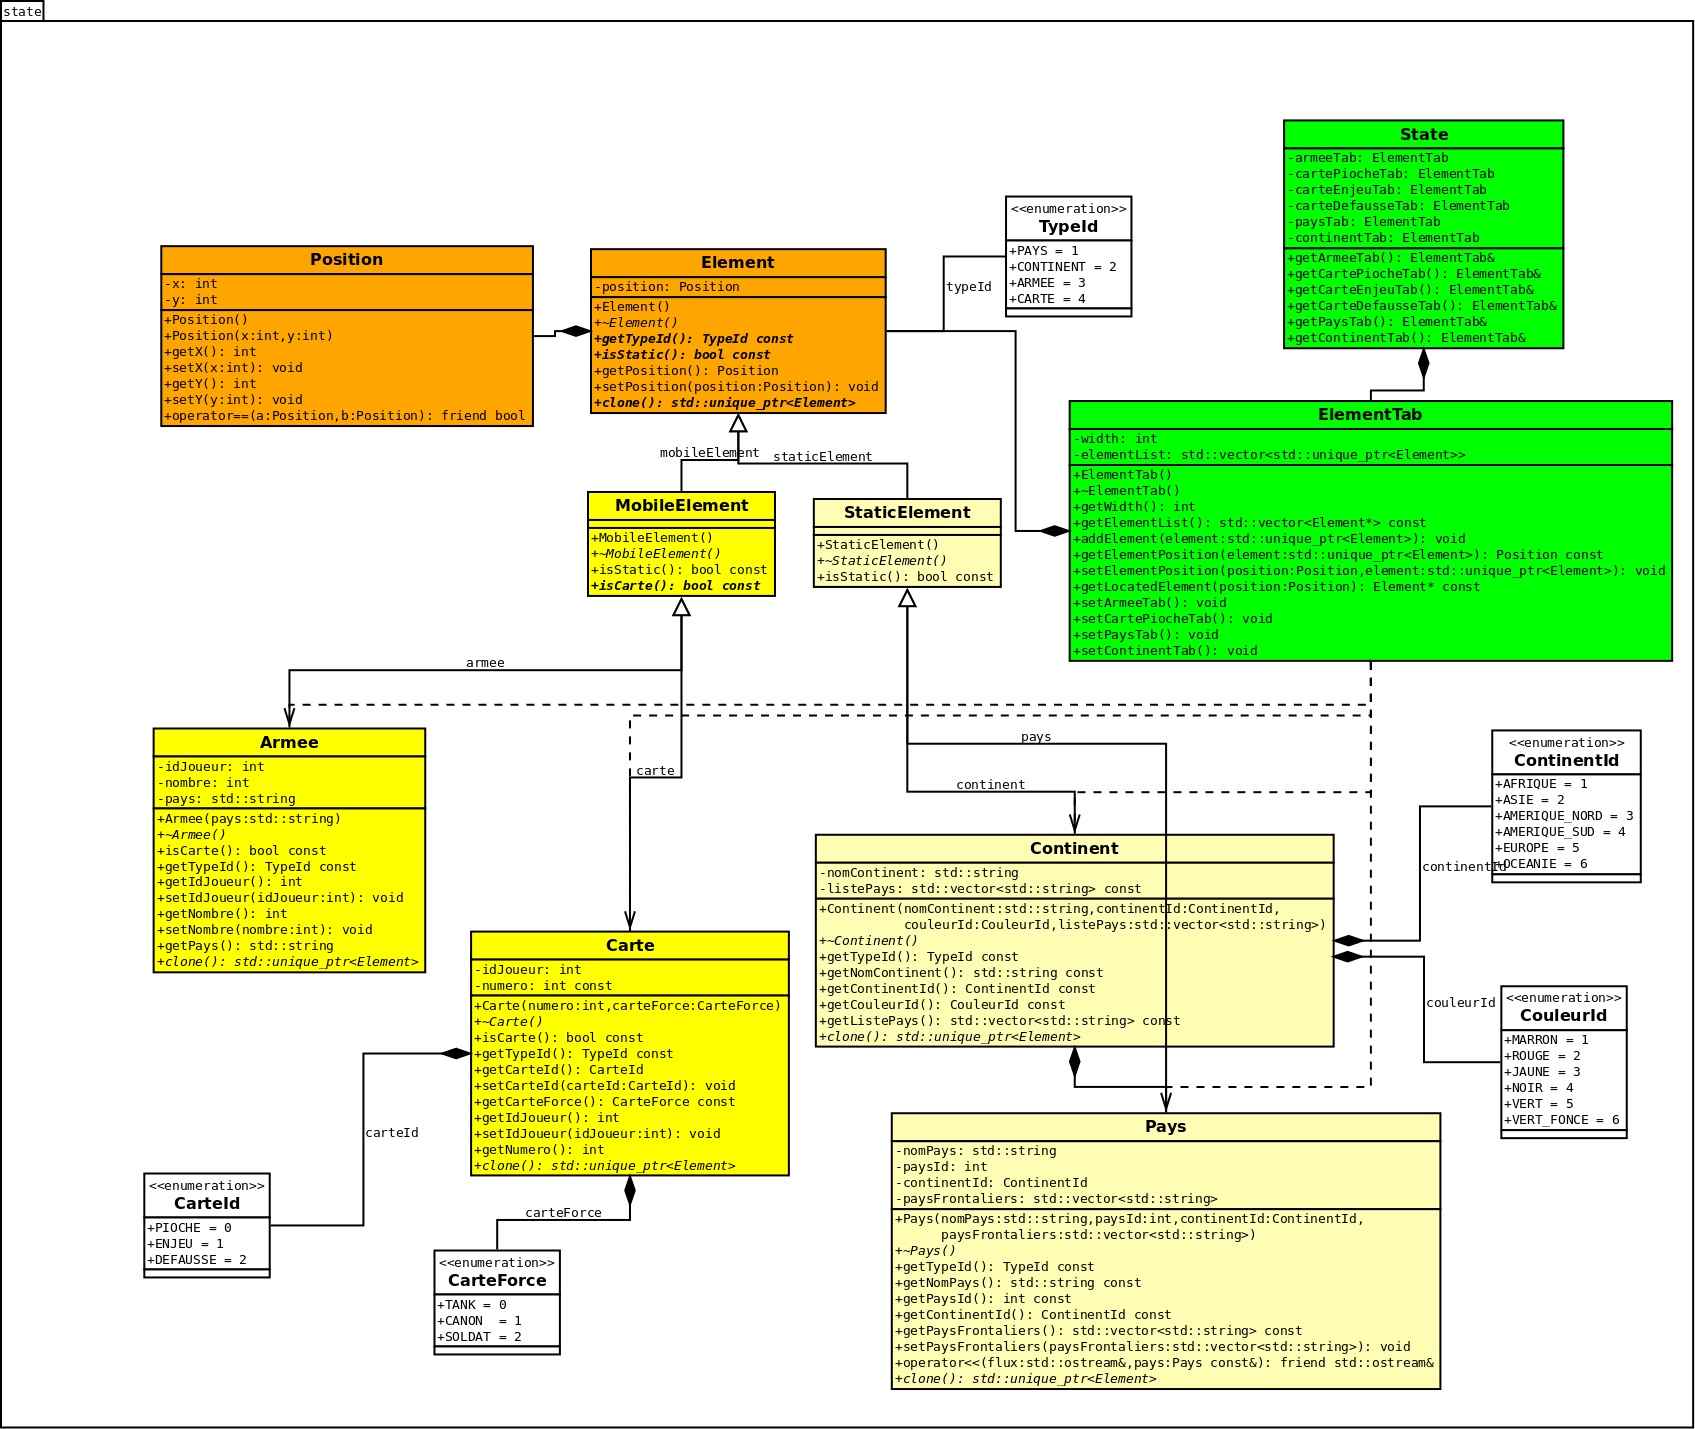
\includegraphics[width=21cm]{Images/state.png}
        \caption{Diagramme des états}
        \label{fig:textures_plateau}
    \end{figure}
\end{landscape}